%!TEX root = main.tex
%%% Graphs and Functions
\part{}

\section{The Rectangular Coordinate System}

\subsection{The \texorpdfstring{$x$-$y$}{x-y} plane}

\begin{center}
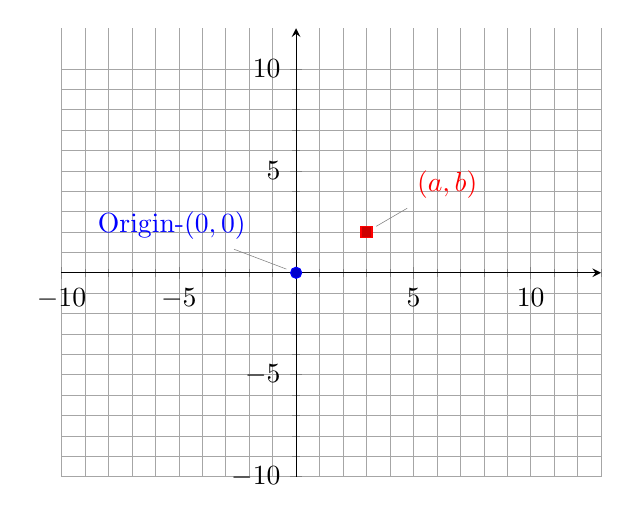
\begin{tikzpicture}
      \begin{axis}%
    [grid=both,
     minor tick num=4,
     grid style={line width=.2pt, draw=gray!70},
     major grid style={line width=.2pt,draw=gray!70},
     axis lines=middle,
     enlargelimits={abs=10}
    ]
    \addplot coordinates {(0,0)} node[pin=150:{Origin-$(0,0)$}]{};
    \addplot coordinates {(3,2)} node[pin=30:{$(a,b)$}]{};
  \end{axis}
\end{tikzpicture}
\end{center}

\begin{exercise}
Find the coordinates of the following points:
\begin{center}
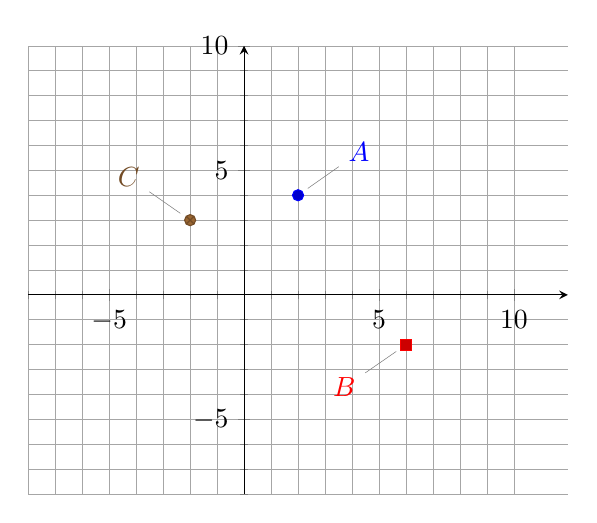
\begin{tikzpicture}
      \begin{axis}%
    [grid=both,
     minor tick num=4,
     grid style={line width=.2pt, draw=gray!70},
     major grid style={line width=.2pt,draw=gray!70},
     axis lines=middle,
     enlargelimits={abs=6}
    ]
    \addplot coordinates {(2,4)} node[pin=30:{$A$}]{};
    \addplot coordinates {(6,-2)} node[pin=210:{$B$}]{};
    \addplot coordinates {(-2,3)} node[pin=150:{$C$}]{};
  \end{axis}
\end{tikzpicture}
\end{center}
\end{exercise}
\begin{solution}[1in]

\end{solution}

\newpage

\subsection{Graphing Lines}

\begin{exercise}
Graph $y=4x-5$ on the $x$-$y$ plane.
\end{exercise}
\ifprintanswers
\else
\begin{center}
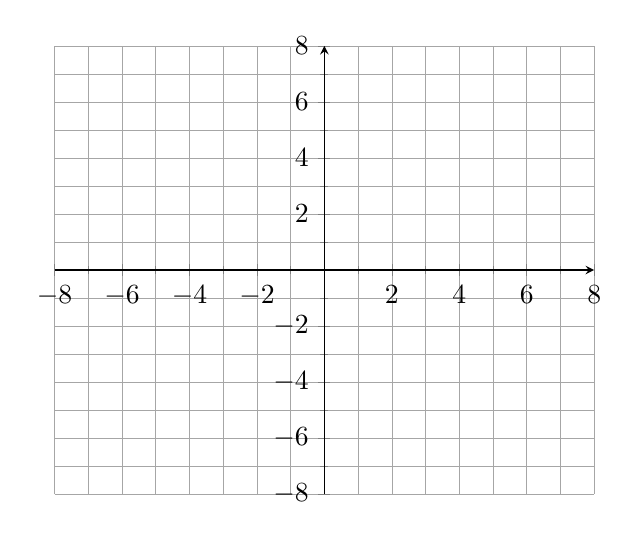
\begin{tikzpicture}
      \begin{axis}%
    [grid=both,
     minor tick num=1,
     grid style={line width=.2pt, draw=gray!70},
     major grid style={line width=.2pt,draw=gray!70},
     xtick={-8,-6,...,6,8},
     ytick={-8,-6,...,6,8},
     xmin=-8, xmax=8,
     ymin=-8, ymax=8,
     axis lines=middle,
     enlargelimits=false
    ]
  \end{axis}
\end{tikzpicture}
\end{center}
\fi
\begin{solution}[2in]

\end{solution}

\begin{exercise}
Graph $y=\frac{4}{3}x-2$ on the $x$-$y$ plane.
\end{exercise}
\ifprintanswers
\else
\begin{center}
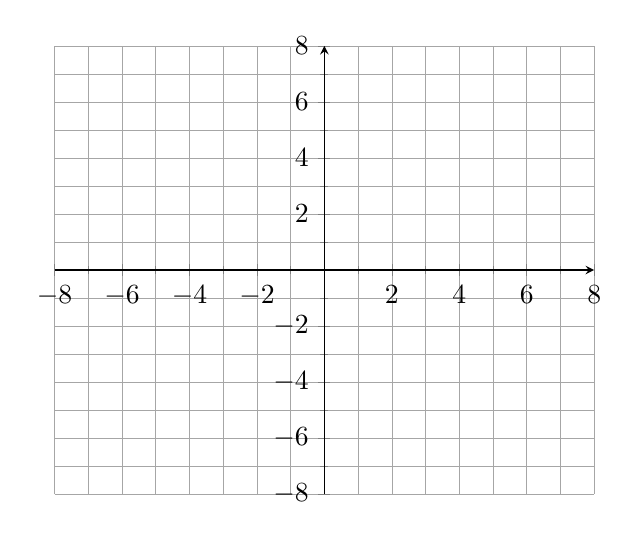
\begin{tikzpicture}
      \begin{axis}%
    [grid=both,
     minor tick num=1,
     grid style={line width=.2pt, draw=gray!70},
     major grid style={line width=.2pt,draw=gray!70},
     xtick={-8,-6,...,6,8},
     ytick={-8,-6,...,6,8},
     xmin=-8, xmax=8,
     ymin=-8, ymax=8,
     axis lines=middle,
     enlargelimits=false
    ]
  \end{axis}
\end{tikzpicture}
\end{center}
\fi
\begin{solution}

\end{solution}

\newpage

\subsection{Distances}

\begin{center}
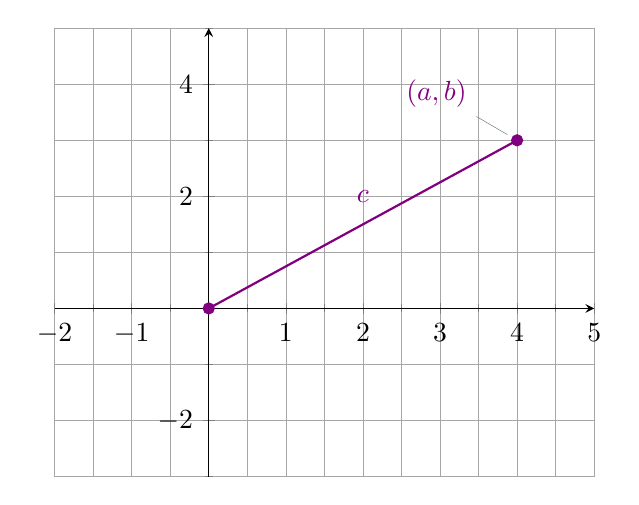
\begin{tikzpicture}
     \begin{axis}%
    [grid=both,
    ymin=-3, ymax=5,
    xmin=-2, xmax=5,
     minor tick num=1,
     grid style={line width=.2pt, draw=gray!70},
     major grid style={line width=.2pt,draw=gray!70},
     axis lines=middle,
     enlargelimits=false
    ]
    \addplot[blue!50!red,only marks] coordinates {(0,0) (4,3)} node[pin=150:{$(a,b)$}]{};
    \addplot[blue!50!red,thick] (0,0) -- (4,3);
    \node[color=blue!50!red] at (2,2) {$c$};
  \end{axis}
\end{tikzpicture}
\end{center}
\begin{ques}
How would we compute the value of $c$ the length of the purple line?
\end{ques}

\subsubsection*{The Pythagorean Theorem}

\begin{theorem}[The Pythagorean Theorem]
Given a right triangle with a hypotenuse of length $c$ and side lengths
$a$ and $b$, then the following holds
\[
\blank{a^2+b^2}{a^2+b^2}=\blank{c^2}{c^2}
\]
\end{theorem}

This means that $c=\blank{\sqrt{a^2+b^2}}{\sqrt{a^2+b^2}}$. Which
is the distance between the points $(0,0)$ \& $(a,b)$.

Looking at it a slightly different way we can say that
\[
c=\blank{\sqrt{(a-0)^2+(b-0)^2}}{(a-0)^2+(b-0)^2}
\]
We can generalize this to the distance between any two points on the plane.

\begin{prop}[The Distance Formula]\label{prop: Distance formula}
Given two points $(x_1,y_1)$ \& $(x_2,y_2)$ in the Cartesian plane, the
distance $D$ between these points is as follows:
\[
D=\blank{\sqrt{(x_2-x_1)^2+(y_2-y_1)^2}}{\sqrt{(x_2-x_1)^2+(y_2-y_1)^2}}
\]
\end{prop}

\begin{exercise}
Find the distance between $(-6,1)$ \& $(5,-1)$.
\end{exercise}
\begin{solution}[2in]

\end{solution}
\vspace{0.5em}

\begin{exercise}
Find the distance between $(2,5)$ \& $(-4,-5)$.
\end{exercise}
\begin{solution}[2in]

\end{solution}
\vspace{0.5em}

\begin{exercise}
Find the distance between $(2,-3)$ \& $(-4,-7)$.
\end{exercise}
\begin{solution}[2in]

\end{solution}
\vspace{0.5em}

\subsection{Midpoints}
\begin{center}
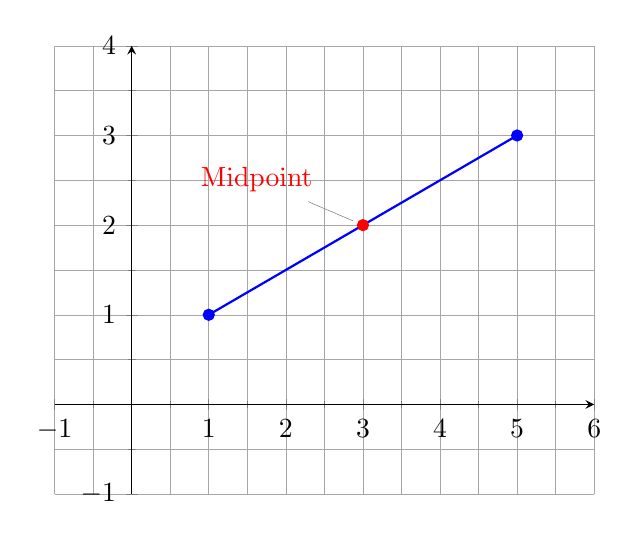
\begin{tikzpicture}
     \begin{axis}%
    [grid=both,
    ymin=-1, ymax=4,
    xmin=-1, xmax=6,
     minor tick num=1,
     grid style={line width=.2pt, draw=gray!70},
     major grid style={line width=.2pt,draw=gray!70},
     axis lines=middle,
     enlargelimits=false
    ]
    \addplot[blue,only marks] coordinates {(1,1) (5,3)};
    \addplot[blue,thick] (1,1) -- (5,3);
    \addplot[red, only marks] coordinates {(3,2)}
    node[pin=150:{Midpoint}]{};
  \end{axis}
\end{tikzpicture}
\end{center}

\begin{definition}
The \emph{midpoint} between two points $(x_1,y_1)$ \& $(x_2,y_2)$
in the Cartesian plane is computed as follows:
\[
\text{Midpoint}=\left(\blank{\frac{x_1+x_2}{2}}{\frac{x_1+x_2}{2}},\blank{\frac{y_1+y_2}{2}}{\frac{y_1+y_2}{2}}\right)
\]
\end{definition}
\vspace{0.5em}

\begin{exercise}
Find the midpoint between $(12,13)$ \& $(-11,7)$.
\end{exercise}
\begin{solution}[2in]

\end{solution}
\vspace{0.5em}

\begin{exercise}
Find the midpoint between $(8,7)$ \& $(12-5)$.
\end{exercise}
\begin{solution}[2in]

\end{solution}
\vspace{0.5em}

\section{Circles}
\begin{center}
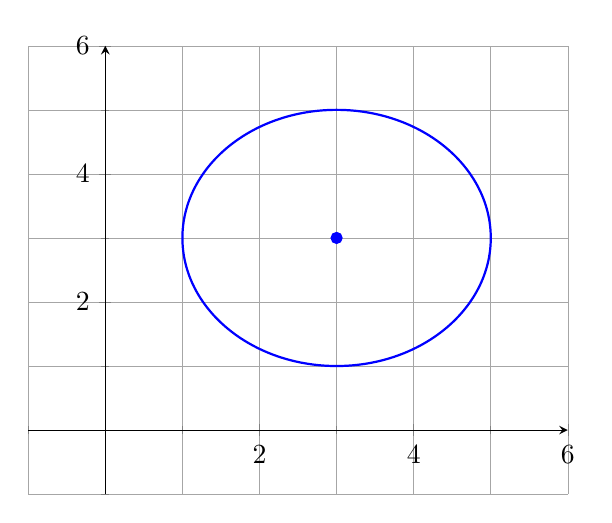
\begin{tikzpicture}
     \begin{axis}%
    [grid=both,
    ymin=-1, ymax=6,
    xmin=-1, xmax=6,
     minor tick num=1,
     xtick = {-2,0,2,...,4,6},
     ytick = {-2,0,2,...,4,6},
     grid style={line width=.2pt, draw=gray!70},
     major grid style={line width=.2pt,draw=gray!70},
     axis lines=middle,
     enlargelimits=false
    ]
    \addplot[blue,only marks] coordinates {(3,3)};
    \draw[color=blue,thick] (axis cs:3,3) circle[radius=2];
  \end{axis}
\end{tikzpicture}
\end{center}

\begin{definition}
A \emph{circle} is a the set of all points $(x,y)$ a distance $r$
from the center $(h,k)$. We call $r$ the \blank{radius}{radius}.
\end{definition}

Using the distance formula (see Proposition
\ref{prop: Distance formula}), we can come up with an equation
for the equation of the a circle as follows
\begin{align*}
\blank{\sqrt{(x-h)^2+(y-k)^2}}{\sqrt{(x-h)^2+(y-k)^2}}&=\blank{r}{r}\\
\blank{(x-h)^2+(y-k)^2}{(x-h)^2+(y-k)^2}&=\blank{r^2}{r^2}\\
\end{align*}

We call this the \emph{standard form of a circle}

\begin{exercise}
Write the following in standard form:
\[
x^2-4x+y^2-2y-31=0
\]
\end{exercise}
\begin{solution}[2in]

\end{solution}
\vspace{0.5em}

\begin{exercise}
Write $2x^2+12x+2y^2+8y-24=0$ in standard form.
\end{exercise}
\begin{solution}[2in]

\end{solution}
\vspace{0.5em}

\newpage

\begin{exercise}
Write the following in standard form:
\[
3x^2-12x+3y^2+6y+3=0
\]
\end{exercise}
\begin{solution}[2in]

\end{solution}
\vspace{0.5em}

\subsection{Graphing circles}

\begin{exercise}
Graph $(x+4)^2+(y+2)^2=16$.
\end{exercise}
\ifprintanswers
\else
\begin{center}
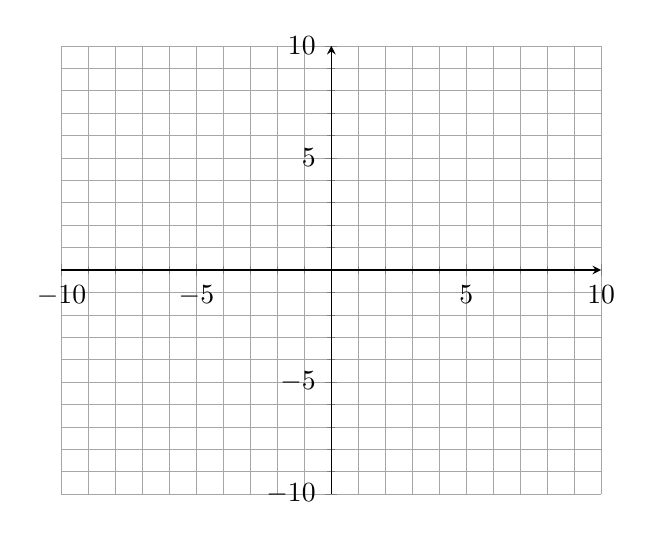
\begin{tikzpicture}
      \begin{axis}%
    [grid=both,
     minor tick num=4,
     grid style={line width=.2pt, draw=gray!70},
     major grid style={line width=.2pt,draw=gray!70},
     xtick={-10,-5,...,5,10},
     ytick={-10,-5,...,5,10},
     xmin=-10, xmax=10,
     ymin=-10, ymax=10,
     axis lines=middle,
     enlargelimits=false
    ]
  \end{axis}
\end{tikzpicture}
\end{center}
\fi
\begin{solution}[2.5in]

\end{solution}

\begin{exercise}
Graph $(x+1)^2+(y-1)^2=4$.
\end{exercise}
\ifprintanswers
\else
\begin{center}
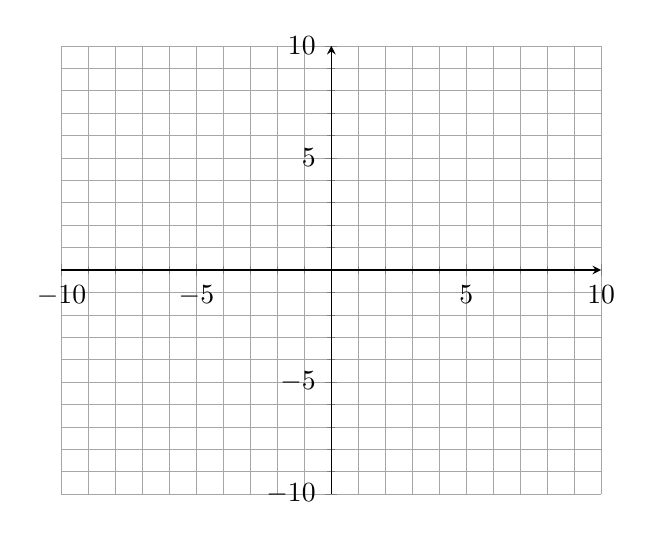
\begin{tikzpicture}
      \begin{axis}%
    [grid=both,
     minor tick num=4,
     grid style={line width=.2pt, draw=gray!70},
     major grid style={line width=.2pt,draw=gray!70},
     xtick={-10,-5,...,5,10},
     ytick={-10,-5,...,5,10},
     xmin=-10, xmax=10,
     ymin=-10, ymax=10,
     axis lines=middle,
     enlargelimits=false
    ]
  \end{axis}
\end{tikzpicture}
\end{center}
\fi
\begin{solution}[2.5in]

\end{solution}

\section{Functions}

\begin{definition}\label{def: relation, domain, range}
A \emph{relation} is any set of order pairs where the \emph{domain}
is the set of \blank{first}{first} values in the ordered pair, and the
\emph{range} is the set of \blank{second}{second} values.
\end{definition}

\begin{exercise}
Find the domain and range of
\[
\{(0,9.1),~(10,6.7),~(20,10.7)\}.
\]
\end{exercise}
\begin{solution}[1.5in]

\end{solution}

\begin{definition}
A \emph{function} is a relation where each element in the domain,
corresponds to exactly one element of the range (i.e. no domain element
can go to two different range elements).
\end{definition}

\begin{example}
$\{(1,2),~(3,4),~(6,5),~(8,5)\}$ is a function
\end{example}

\begin{nonex}
$\{(1,2),~(3,4),~(5,6),~(5,8)\}$ is a NOT function
\end{nonex}

\subsection{Equations as functions}

\begin{definition}\label{def: independent dependent variables}
We will call $\blank{x}{x}$ the \emph{independent variable}
which corresponds to the \blank{domain}{domain}, and we will
call $\blank{y}{y}$ the $\emph{dependent variable}$ which
corresponds to the \blank{range}{range}.
\end{definition}

\begin{note}
This means that an equation is a functions if every $\blank{x}{x}$
goes to exactly one $\blank{y}{y}$.
\end{note}

\begin{exercise}
Is $2x+y=6$ a function?
\end{exercise}
\begin{solution}[1in]

\end{solution}

\begin{exercise}
Is $x^2+y^2=1$ a function?
\end{exercise}
\begin{solution}[1in]

\end{solution}

\subsection{Function Notation}

\begin{example}
We can rewrite the function $y=x^2-2x+7$, in \emph{function notation},
as follows:
\[
f(x)=x^2-2x+7
\]
We read $f(x)$ as ``$f$ of $x$'', so $f(-)$ is ``$f$ of $-$''
\end{example}

Function notation is useful if in evaluation.

\begin{exercise}
For $f(x)=x^2-2x+7$, find $f(-5)$.
\end{exercise}
\begin{solution}[1in]

\end{solution}

\begin{exercise}
For $f(x)=x^2-2x+7$, find $f(2)$.
\end{exercise}
\begin{solution}[2in]

\end{solution}

\begin{exercise}
For $f(x)=x^2-2x+7$, find $f(x+4)$.
\end{exercise}
\begin{solution}[2in]

\end{solution}

\subsubsection*{Solving using function notation}

\begin{exercise}
For $f(a)=4a^2-29a$, solve $f(a)=-30$.
\end{exercise}
\begin{solution}[2.5in]

\end{solution}

\newpage

\begin{exercise}
Find when $h(x)=-12$ if $h(x)=x^2-7x$.
\end{exercise}
\begin{solution}[2in]

\end{solution}

\subsection{Graphing Functions}

Recall that ``$f(x)=$'' $\leftrightarrow$ ``$y=$'', so the output of
a function is the $y$-value.

\begin{exercise}
Graph $f(x)=2x+1$.
\end{exercise}
\ifprintanswers
\else
\begin{center}
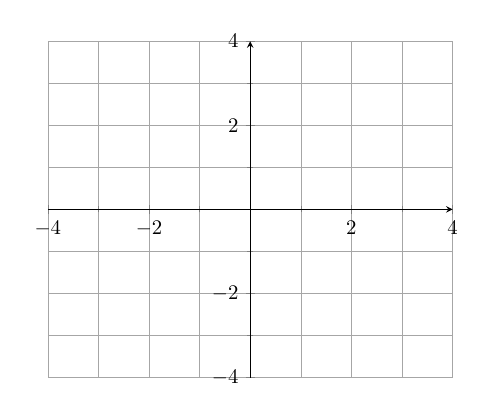
\begin{tikzpicture}[scale=0.75]
      \begin{axis}%
    [grid=both,
     minor tick num=1,
     grid style={line width=.2pt, draw=gray!70},
     major grid style={line width=.2pt,draw=gray!70},
     xtick={-4,-2,...,2,4},
     ytick={-4,-2,...,2,4},
     xmin=-4, xmax=4,
     ymin=-4, ymax=4,
     axis lines=middle,
     enlargelimits=false
    ]
  \end{axis}
\end{tikzpicture}
\end{center}
\fi

\begin{note}
Every function has a graph, but not every graph has a function.
\end{note}

\subsubsection{Vertical Line Test}
\begin{prop}[Vertical line test]
If any vertical line crosses a graph more than once, it does not represent a function.
\end{prop}
\begin{center}
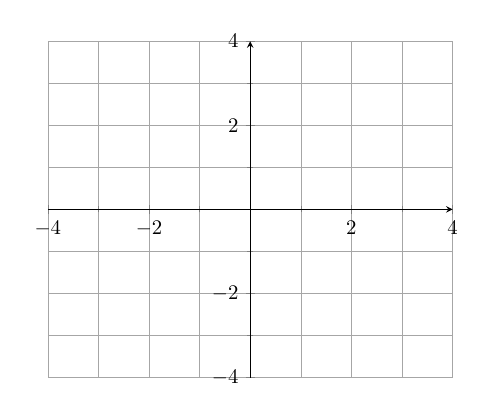
\begin{tikzpicture}[scale=0.75]
      \begin{axis}%
    [grid=both,
     minor tick num=1,
     grid style={line width=.2pt, draw=gray!70},
     major grid style={line width=.2pt,draw=gray!70},
     xtick={-4,-2,...,2,4},
     ytick={-4,-2,...,2,4},
     xmin=-4, xmax=4,
     ymin=-4, ymax=4,
     axis lines=middle,
     enlargelimits=false
    ]
  \end{axis}
\end{tikzpicture}
\hspace{1in}
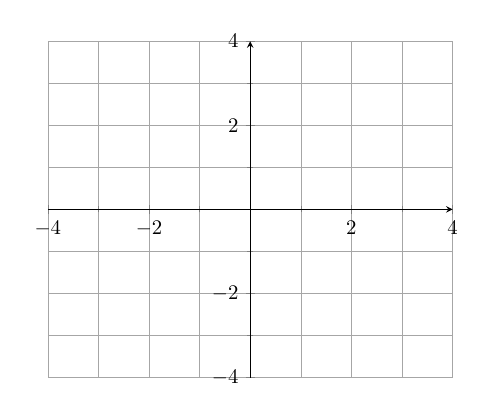
\begin{tikzpicture}[scale=0.75]
      \begin{axis}%
    [grid=both,
     minor tick num=1,
     grid style={line width=.2pt, draw=gray!70},
     major grid style={line width=.2pt,draw=gray!70},
     xtick={-4,-2,...,2,4},
     ytick={-4,-2,...,2,4},
     xmin=-4, xmax=4,
     ymin=-4, ymax=4,
     axis lines=middle,
     enlargelimits=false
    ]
  \end{axis}
\end{tikzpicture}
\end{center}

Here are some other symbols to be familiar with:
\begin{itemize}
    \item \blank{open dot}{open dot} - ends at that point, but does
    NOT include it.
    \item \blank{closed dot}{closed dot} - ends at that point AND includes it.
    \item \blank{arrow}{arrow} - the graph continues in that direction forever.
\end{itemize}

\subsection{Finding Domain and Range from a Graph}

\begin{exercise}
Find the domain and range of the following:
\begin{center}
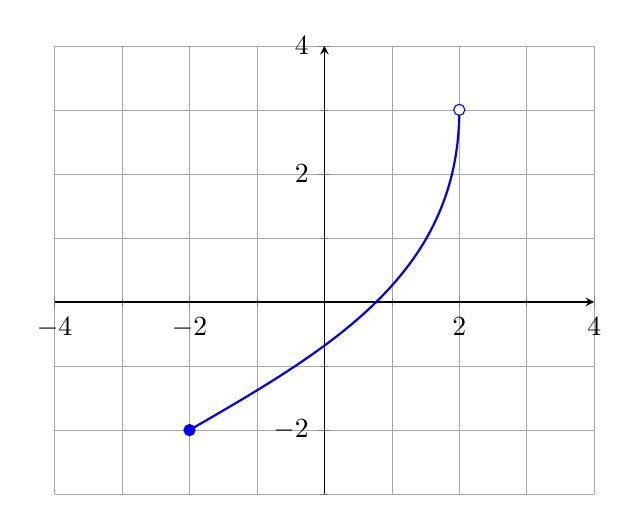
\begin{tikzpicture}
     \begin{axis}%
    [grid=both,
    ymin=-3, ymax=4,
    xmin=-4, xmax=4,
     minor tick num=1,
     grid style={line width=.2pt, draw=gray!70},
     major grid style={line width=.2pt,draw=gray!70},
     axis lines=middle,
     enlargelimits=false
    ]
    \addplot[blue,only marks] coordinates {(-2,-2)};
    \addplot[blue,mark=*,fill=white] coordinates {(2,3)};
    \addplot[blue,smooth,thick] (-2,-2) to[out=30, in=-90] (2,3);
  \end{axis}
\end{tikzpicture}
\end{center}
\end{exercise}
\begin{solution}[0.75in]

\end{solution}

\begin{exercise}
Find the domain and range of the following:
\begin{center}
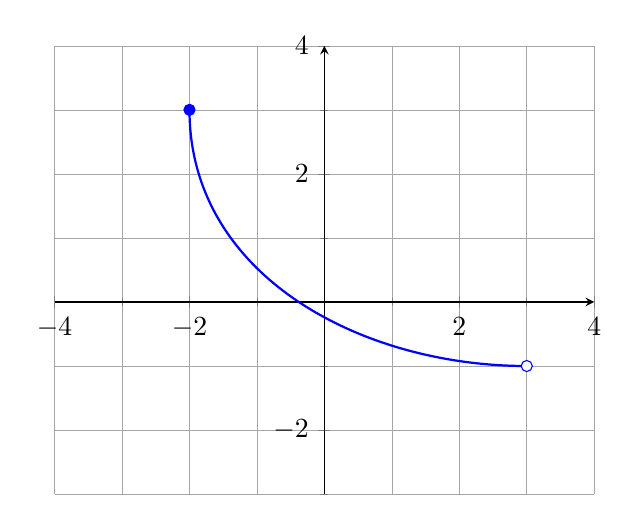
\begin{tikzpicture}
     \begin{axis}%
    [grid=both,
    ymin=-3, ymax=4,
    xmin=-4, xmax=4,
     minor tick num=1,
     grid style={line width=.2pt, draw=gray!70},
     major grid style={line width=.2pt,draw=gray!70},
     axis lines=middle,
     enlargelimits=false
    ]
    \addplot[blue,only marks] coordinates {(-2,3)};
    \addplot[blue,mark=*,fill=white] coordinates {(3,-1)};
    \addplot[blue,smooth,thick] (-2,3) to[out=-90, in=180] (3,-1);
  \end{axis}
\end{tikzpicture}
\end{center}
\end{exercise}
\begin{solution}[=0.75in]

\end{solution}

\begin{exercise}
Find the domain and range of the following:
\begin{center}
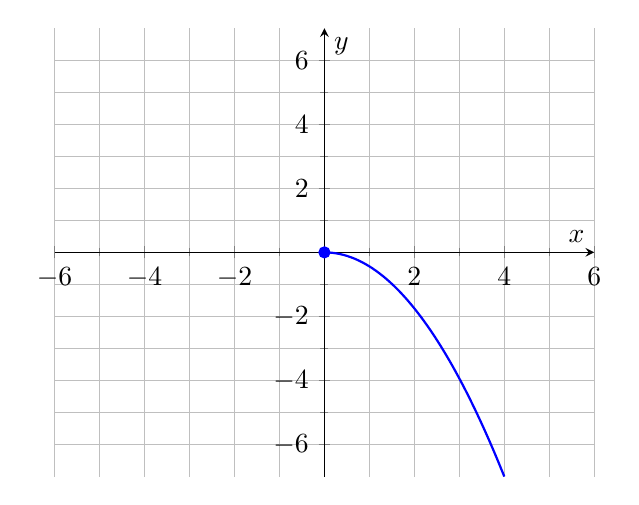
\begin{tikzpicture}
     \begin{axis}%
    [grid=both,
    minor tick num=1,
    axis x line=middle, axis y line=middle,
    ymin=-7, ymax=7, ytick={-6,-4,...,4,6}, ylabel=$y$,
    xmin=-6, xmax=6, xtick={-6,-4,...,4,6}, xlabel=$x$
    ]
    \addplot[blue,mark=*] coordinates {(0,0)};
    \addplot+[blue,smooth,thick,domain=0:4,mark=none] {-7/16*x^2};
  \end{axis}
\end{tikzpicture}
\end{center}
\end{exercise}
\begin{solution}[1in]

\end{solution}
\vspace{0.5em}

\begin{exercise}
Find the domain and range of the function shown below:
\begin{center}
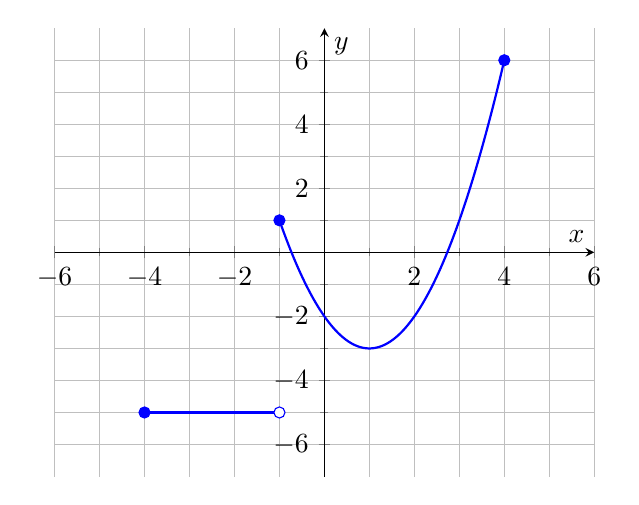
\begin{tikzpicture}
     \begin{axis}%
    [grid=both,
    minor tick num=1,
    axis x line=middle, axis y line=middle,
    ymin=-7, ymax=7, ytick={-6,-4,...,4,6}, ylabel=$y$,
    xmin=-6, xmax=6, xtick={-6,-4,...,4,6}, xlabel=$x$
    ]
    \addplot+[blue,mark=none,thick,domain=-1:4,
     samples=100,] {x^2-2*x-2};
    \addplot[blue,mark=none,thick] (-4,-5)--(-1,-5);
    \addplot[blue,mark=*,only marks] coordinates {(-4,-5) (-1,1) (4,6)};
    \addplot[blue,mark=*,fill=white,only marks] coordinates {(-1,-5)};
  \end{axis}
\end{tikzpicture}
\end{center}
\end{exercise}
\begin{solution}[2in]

\end{solution}
\vspace{0.5em}

\subsection{Finding domains from equations}

For some of these questions instead of asking what numbers work, the easier
question is what numbers ``don't work''.

\begin{exercise}
Find the domain of
\[
f(x)=\frac{1}{(x+3)(x-2)}
\]
\end{exercise}
\begin{solution}[2in]

\end{solution}
\vspace{0.5em}

\begin{exercise}
Find the domain of
\[
g(x)=\sqrt{x+2}
\]
\end{exercise}
\begin{solution}[1.5in]

\end{solution}
\vspace{0.5em}

\begin{exercise}
Find the domain of
\[
q(x)=\frac{1}{\sqrt{8-9x}}
\]
\end{exercise}
\begin{solution}[2in]

\end{solution}
\vspace{0.5em}

\section{Linear Functions}

\subsection{Slope}

\begin{definition}
The \emph{slope} of a line is the following ratio
\[
m=\frac{\emptyfrac{\text{rise}}}{\emptyfrac{\text{run}}}=\frac{\emptyfrac{\text{Change in }y}}{\emptyfrac{\text{Change in }x}}
\]
If $(x_1,y_1)$ \& $(x_2,y_2)$ are two points on a line, then the slope is
\[
m=\frac{\emptyfrac{y_2-y_1}}{\emptyfrac{x_2-x_1}}
\]
\end{definition}
\vspace{0.5em}

\begin{exercise}
Find the slope of the line between $(-3,4)$ \& $(-4,-2)$.
\end{exercise}
\begin{solution}[1in]

\end{solution}
\vspace{0.5em}

\begin{exercise}
Find the slope of the line between $(4,-2)$ \& $(-1,5)$.
\end{exercise}
\begin{solution}[1in]

\end{solution}
\vspace{0.5em}

\begin{exercise}
Find the slope of the line between $(7,-3)$ \& $(1,11)$.
\end{exercise}
\begin{solution}[1in]

\end{solution}
\vspace{0.5em}

\subsection{Graphs}

\vspace{3em}

\ifprintanswers
\else
\begin{center}
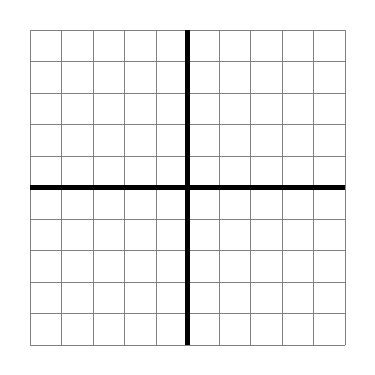
\begin{tikzpicture}[scale=0.4]
\draw[step=1cm,gray,very thin] (-5,-5) grid (5,5);
\draw[black,ultra thick] (-5,0) -- (5,0);
\draw[black,ultra thick] (0,-5) -- (0,5);
\end{tikzpicture}
\hspace{2in}
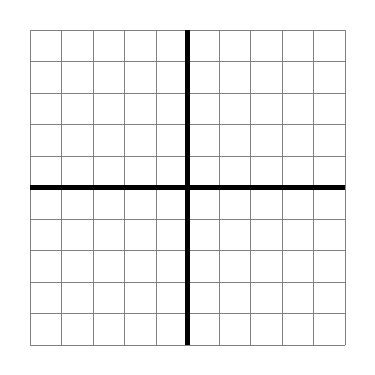
\begin{tikzpicture}[scale=0.4]
\draw[step=1cm,gray,very thin] (-5,-5) grid (5,5);
\draw[black,ultra thick] (-5,0) -- (5,0);
\draw[black,ultra thick] (0,-5) -- (0,5);
\end{tikzpicture}

\vspace{5em}

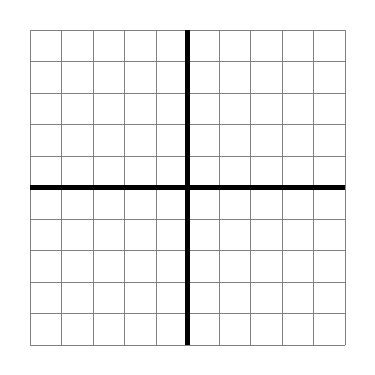
\begin{tikzpicture}[scale=0.4]
\draw[step=1cm,gray,very thin] (-5,-5) grid (5,5);
\draw[black,ultra thick] (-5,0) -- (5,0);
\draw[black,ultra thick] (0,-5) -- (0,5);
\end{tikzpicture}
\hspace{2in}
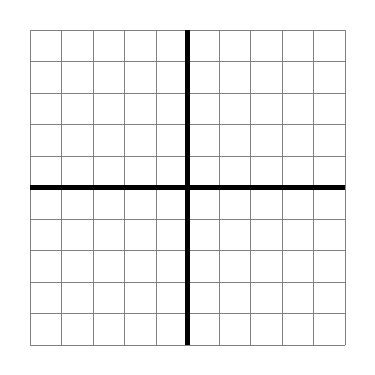
\begin{tikzpicture}[scale=0.4]
\draw[step=1cm,gray,very thin] (-5,-5) grid (5,5);
\draw[black,ultra thick] (-5,0) -- (5,0);
\draw[black,ultra thick] (0,-5) -- (0,5);
\end{tikzpicture}
\end{center}
\fi

\subsubsection{Slope-Intercept form}

\vspace{0.5em}

\begin{center}
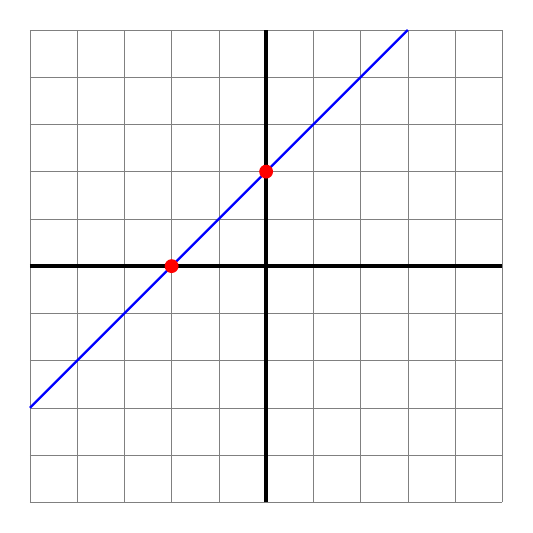
\begin{tikzpicture}[scale=0.6]
\draw[step=1cm,gray,very thin] (-5,-5) grid (5,5);
\draw[black,ultra thick] (-5,0) -- (5,0);
\draw[black,ultra thick] (0,-5) -- (0,5);

\draw[blue,thick] (-5,-3) -- (3,5);
\node[circle,fill=red,inner sep=0pt,minimum size=5pt](x) at (-2,0) {};
\node[circle,fill=red,inner sep=0pt,minimum size=5pt](y) at (0,2) {};
\end{tikzpicture}   
\end{center}

\vspace{0.5em}

\begin{definition}[Slope-intercept form]\label{def: slope-intercept form}
A line with slope $m$ and $y$-intercept $b$ has the equation
\[
y=\blank{mx+b}{mx+b}
\]
\end{definition}

\vspace{0.5em}

\begin{exercise}
What are the slope and $y$-intercept of $y=3x-4$?
\end{exercise}
\begin{solution}[1in]

\end{solution}

\begin{exercise}
What is the $x$ intercept of $f(x)=2x-8$?
\end{exercise}
\begin{solution}[1in]

\end{solution}

\begin{exercise}
Find the slope-intercept form of the line with slope $7$ and $y$-intercept $2$.
\end{exercise}
\begin{solution}[1in]

\end{solution}

\subsection{Graphing Lines}
\begin{exercise}
Graph $f(x)=2x+5$
\end{exercise}
\ifprintanswers
\else
\begin{center}
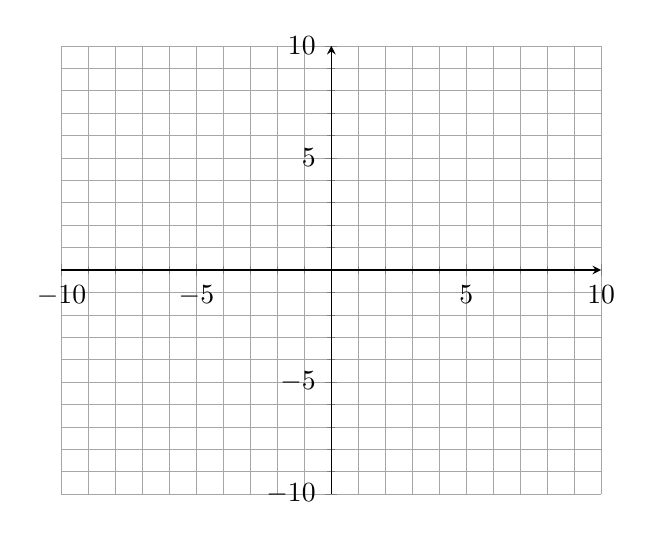
\begin{tikzpicture}
      \begin{axis}%
    [grid=both,
     minor tick num=4,
     grid style={line width=.2pt, draw=gray!70},
     major grid style={line width=.2pt,draw=gray!70},
     xtick={-10,-5,...,5,10},
     ytick={-10,-5,...,5,10},
     xmin=-10, xmax=10,
     ymin=-10, ymax=10,
     axis lines=middle,
     enlargelimits=false
    ]
  \end{axis}
\end{tikzpicture}       
\end{center}
\fi

\newpage

\begin{exercise}
Graph $h(x)=-3x-6$
\end{exercise}
\ifprintanswers
\else
\begin{center}
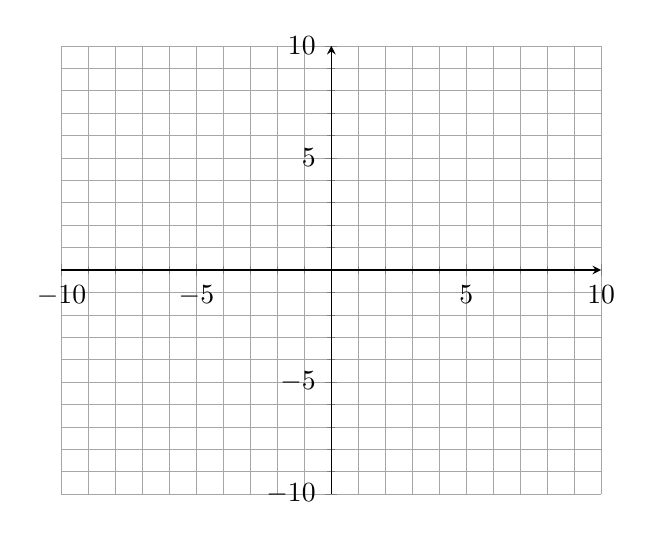
\begin{tikzpicture}
      \begin{axis}%
    [grid=both,
     minor tick num=4,
     grid style={line width=.2pt, draw=gray!70},
     major grid style={line width=.2pt,draw=gray!70},
     xtick={-10,-5,...,5,10},
     ytick={-10,-5,...,5,10},
     xmin=-10, xmax=10,
     ymin=-10, ymax=10,
     axis lines=middle,
     enlargelimits=false
    ]
  \end{axis}
\end{tikzpicture} 
\end{center}
\fi

\begin{exercise}
Find $y=mx+b$ for the following:
\begin{center}
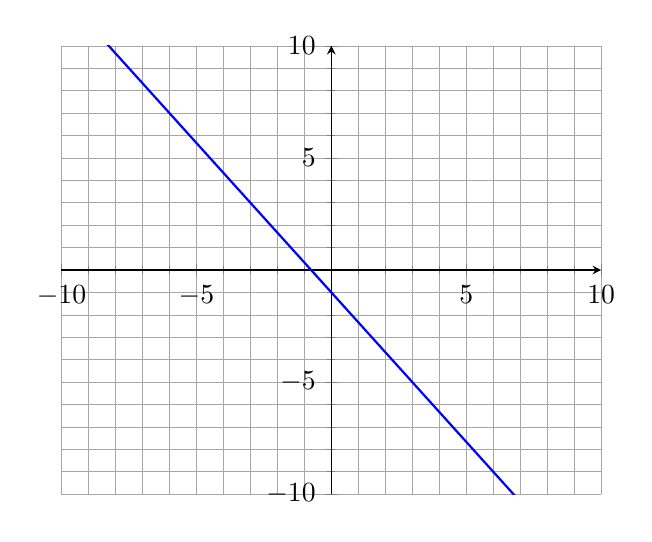
\begin{tikzpicture}
      \begin{axis}%
    [grid=both,
     minor tick num=4,
     grid style={line width=.2pt, draw=gray!70},
     major grid style={line width=.2pt,draw=gray!70},
     xtick={-10,-5,...,5,10},
     ytick={-10,-5,...,5,10},
     xmin=-10, xmax=10,
     ymin=-10, ymax=10,
     axis lines=middle,
     enlargelimits=false
    ]
      \addplot[blue,thick,domain=-10:10] {-4/3*x-1};
  \end{axis}
\end{tikzpicture}
\end{center}
\end{exercise}

\section{More on Lines}

\subsection{Finding the equation of a line}

In general, to find the equation of a line we need the slope and any point on the line.

\vspace{0.5em}

\begin{definition}[Point-slope form]\label{def: point slope form}
If we have a point $(x_1,y_1)$ on a line with slope $m$, then the \emph{point-slope form} is
\[
\blank{y-y_1}{y-y_1}=\blank{m(x-x_1)}{m(x-x_1)}
\]
\end{definition}

\newpage

\begin{exercise}
Find the equation of a line passing through $(2,-5)$ with slope $m=6$ in slope-intercept form.
\end{exercise}
\begin{solution}[3in]

\end{solution}

\begin{exercise}
Find the equation of a line passing through $(3,4)$ with slope $m=-5$ in slope-intercept form.
\end{exercise}
\begin{solution}[2in]

\end{solution}

\begin{exercise}
Find the equation of a line passing through $(3,4)$ \& $(-1,-6)$ in slope-intercept form.
\end{exercise}
\begin{solution}[2in]

\end{solution}

\subsection{Standard Form}

\begin{definition}[Standard form]\label{def: standard from of a line}
If $A$, $B$, and $C$ are integers (with $A>0$), then the standard form of a line is
\[
\blank{Ax+By}{Ax+By}=\blank{C}{C}\quad\text{or}\quad\blank{Ax+By+C}{Ax+By+C}=\blank{0}{0}
\]
\end{definition}

\begin{exercise}
Find the standard form of the line passing through $(-8,-1)$ \& $(-1,-2)$.
\end{exercise}
\begin{solution}[2in]

\end{solution}

\begin{exercise}
Find the standard form of the line passing through $(-7,-4)$ \& $(-2,3)$.
\end{exercise}
\begin{solution}[2in]

\end{solution}

\subsection{Horizontal \& Vertical Lines}

\begin{note}
A horizontal line has a slope of \blank{0}{0}. This means that their equation
is
\[
y=\blank{0x+b}{0x+b}=\blank{0+b}{0+b}=\blank{b}{b}
\]
Every horizontal line can be written this way, which makes sense because the
\blank{$y$-value}{$y$-value} never changes.
\end{note}

\vspace{0.5em}

\begin{note}
In a similar way, the \blank{$x$-value}{$x$-value} never changes for vertical lines,
their equation looks like
\[
\blank{x}{x}=\blank{a}{a}
\]
\end{note}

\vspace{0.5em}

\begin{exercise}
What is the equation of the following line?
\begin{center}
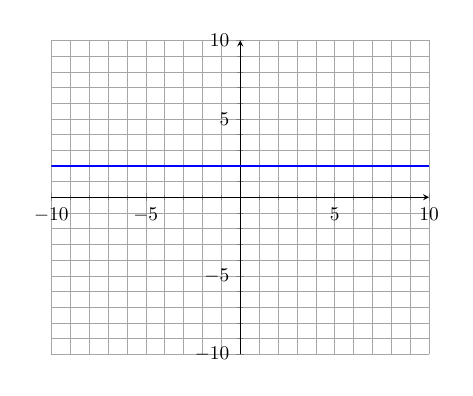
\begin{tikzpicture}[scale=.7]
      \begin{axis}%
    [grid=both,
     minor tick num=4,
     grid style={line width=.2pt, draw=gray!70},
     major grid style={line width=.2pt,draw=gray!70},
     xtick={-10,-5,...,5,10},
     ytick={-10,-5,...,5,10},
     xmin=-10, xmax=10,
     ymin=-10, ymax=10,
     axis lines=middle,
     enlargelimits=false
    ]
      \addplot[blue,thick,domain=-10:10] {2};
  \end{axis}
\end{tikzpicture}  
\end{center}
\end{exercise}

\vspace{0.5em}

\begin{exercise}
What is the equation of the following line?
\begin{center}
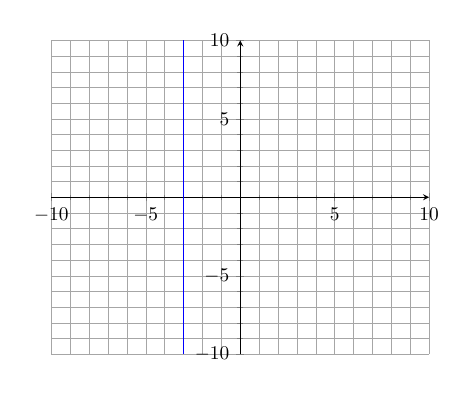
\begin{tikzpicture}[scale=.7]
      \begin{axis}%
    [grid=both,
     minor tick num=4,
     grid style={line width=.2pt, draw=gray!70},
     major grid style={line width=.2pt,draw=gray!70},
     xtick={-10,-5,...,5,10},
     ytick={-10,-5,...,5,10},
     xmin=-10, xmax=10,
     ymin=-10, ymax=10,
     axis lines=middle,
     enlargelimits=false
    ]
     \draw[blue,thick] (-3,-10) -- (-3,10);
  \end{axis}
\end{tikzpicture}
\end{center}
\end{exercise}

\subsection{Parallel and Perpendicular Lines}

\begin{definition}\label{def: Parallel lines}
Two lines are called \emph{parallel} (denoted by $\parallel$) 
if they \blank{never intersect}{never intersect}
\end{definition}

\begin{prop}\label{prop: parallel line conditions}
\text{}
\begin{itemize}
    \item Two distinct non-vertical lines are parallel if and only if
   \blank{they have the same slope}{they have the same slope}.
   \item If two vertical lines are \blank{distinct}{distinct}, then
   they are parallel.
\end{itemize}
\end{prop}

\begin{exercise}
Find the slope-intercept form of a line passing through $(-2,5)$
and parallel to $y=3x+1$.
\end{exercise}
\begin{solution}[2in]

\end{solution}

\newpage

\begin{exercise}
Find the line parallel to $y=5x-9$ passing through $(4,-2)$ in slope-intercept form.
\end{exercise}
\begin{solution}[2in]

\end{solution}

\begin{definition}
Two lines are called \emph{perpendicular} (denoted by $\perp$) if they
\blank{intersect at a $90^\circ$}{intersect at a $90^\circ$}.
\end{definition}

\begin{prop}\label{prop: perp line conditions}
\text{}
\begin{itemize}
    \item Two distinct non-vertical lines are perpendicular if and only if the
    product of their slopes is \blank{$-1$}{$-1$}.
   \item Horizontal and vertical lines are \blank{always}{always} perpendicular.
\end{itemize}
\end{prop}

\begin{note}
Another way to understand the first point is if the one slope is $m=\frac{a}{b}$,
then the perpendicular slope is $m_\perp=\blank{-\frac{b}{a}}{-\frac{b}{a}}$
\end{note}

\begin{exercise}
Find a line through $(-2,-6)$ and perpendicular to $y=-\frac{1}{3}x+4$ in slope-intercept form.
\end{exercise}
\begin{solution}[2in]

\end{solution}

\newpage

\begin{exercise}
Find the equation of the line perpendicular to $y=\frac{1}{4}x-4$
and passing through $(-8,5)$ in slope-intercept form.
\end{exercise}
\begin{solution}[2in]

\end{solution}

\vspace{0.5em}

\begin{exercise}
Are the following two lines parallel, perpendicular, or neither?
\[
y=3x-5\quad y+\frac{1}{3}x=2
\]
\end{exercise}
\begin{solution}[1.5in]

\end{solution}

\subsection{Real-World Applications}

\begin{exercise}
You are considering using a moving company to help you move. They charge \$60 per hour
plus a base fee of \$290. If $C$ is the total cost of hiring the moving company and $H$
is the number of hours worked, what is the relationship between $H$ and $C$?
\end{exercise}
\begin{solution}[3in]

\end{solution}

\section{Transformations of Graphs/Functions}

\subsection{The Basic Transformations}

Let $f(x)$ be a function. Then there are 4 (or 6) basic transformations:

\begin{enumerate}[1)]
\item Vertical Shifts
\[
\blank{f(x)\pm c}{f(x)\pm c}
\]
\vspace{1.5em}

\item Horizontal Shifts
\[
\blank{f(x\pm c)}{f(x\pm c)}
\]
\vspace{3em}

\item Vertical stretches \& shrinks/compressions
\[
\blank{cf(x)}{cf(x)}
\]
\vspace{3em}

\begin{enumerate}[3.5)]
\item Vertical ($x$-axis) Reflection
\[
\blank{-1f(x)}{-1f(x)}
\]
\end{enumerate}

\vspace{3em}

\item Horizontal stretches \& shrinks/compressions
\[
\blank{f(c x)}{f(c x)}
\]
\vspace{3em}
\begin{enumerate}[4.5)]
\item Horizontal ($y$-axis) Reflection
\[
\blank{f(-1x)}{f(-1x)}
\]
\vspace{3em}
\end{enumerate}
\end{enumerate}

\newpage

\begin{example}
Vertical shift: Transform $f(x)$ to $f(x)+2$
\end{example}
\ifprintanswers
\else
\begin{center}
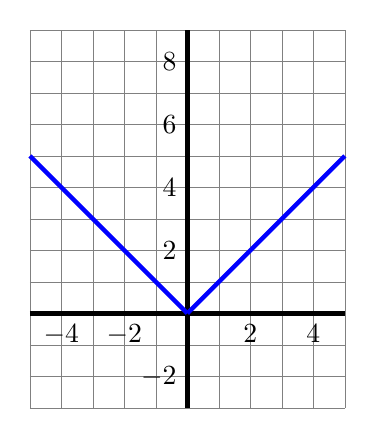
\begin{tikzpicture}[scale=0.4]
\draw[step=1cm,gray,very thin] (-5,-3) grid (5,9);
\draw[black,ultra thick] (-5,0) -- (5,0);
\draw[black,ultra thick] (0,-3) -- (0,9);

\foreach\x/\xtext in {-4,-2,2,4}
\draw (\x ,1pt) -- (\x,-1pt) node[anchor=north] {$\xtext$};
\foreach\y/\ytext in {-2,2,4,6,8}
\draw (1pt,\y) -- (-1pt,\y) node[anchor=east] {$\ytext$};
\draw[blue,ultra thick] (-5,5) -- (0,0);
\draw[blue,ultra thick] (5,5) -- (0,0);
\end{tikzpicture}
\end{center}
\fi

\begin{example}
Horizontal shift: Find $f(x+3)$ using $f(x)$ below
\end{example}
\ifprintanswers
\else
\begin{center}
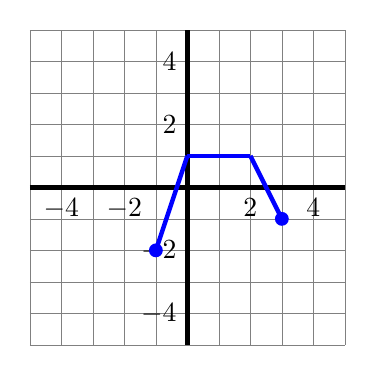
\begin{tikzpicture}[scale=0.4]
\draw[step=1cm,gray,very thin] (-5,-5) grid (5,5);
\draw[black,ultra thick] (-5,0) -- (5,0);
\draw[black,ultra thick] (0,-5) -- (0,5);

\foreach\x/\xtext in {-4,-2,2,4}
\draw (\x ,1pt) -- (\x,-1pt) node[anchor=north] {$\xtext$};
\foreach\y/\ytext in {-4,-2,2,4}
\draw (1pt,\y) -- (-1pt,\y) node[anchor=east] {$\ytext$};
\draw[blue,ultra thick] (-1,-2) -- (0,1);
\draw[blue,ultra thick] (0,1) -- (2,1);
\draw[blue,ultra thick] (2,1) -- (3,-1);
\node[circle,fill=blue,inner sep=0pt,minimum size=5pt](x) at (-1,-2) {};
\node[circle,fill=blue,inner sep=0pt,minimum size=5pt](y) at (3,-1) {};
\end{tikzpicture}
\end{center}
\fi

\begin{example}
Vertical Stretch \& Shrink/Compression: Find $3f(x)$ using $f(x)$ below
\end{example}
\ifprintanswers
\else
\begin{center}
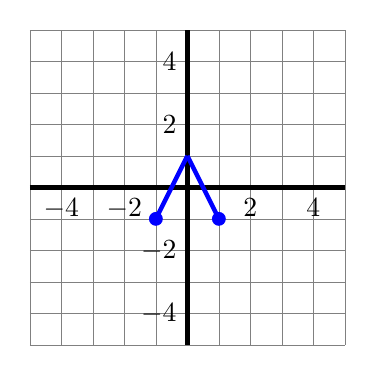
\begin{tikzpicture}[scale=0.4]
\draw[step=1cm,gray,very thin] (-5,-5) grid (5,5);
\draw[black,ultra thick] (-5,0) -- (5,0);
\draw[black,ultra thick] (0,-5) -- (0,5);

\foreach\x/\xtext in {-4,-2,2,4}
\draw (\x ,1pt) -- (\x,-1pt) node[anchor=north] {$\xtext$};
\foreach\y/\ytext in {-4,-2,2,4}
\draw (1pt,\y) -- (-1pt,\y) node[anchor=east] {$\ytext$};
\draw[blue,ultra thick] (-1,-1) -- (0,1);
\draw[blue,ultra thick] (0,1) -- (1,-1);
\node[circle,fill=blue,inner sep=0pt,minimum size=5pt](x) at (-1,-1) {};
\node[circle,fill=blue,inner sep=0pt,minimum size=5pt](y) at (1,-1) {};
\end{tikzpicture}
\end{center}
\fi

\begin{example}
Horizontal Stretch \& Shrink/Compression:
Find $f(-2x)$ using $f(x)$ below
\end{example}
\ifprintanswers
\else
\begin{center}
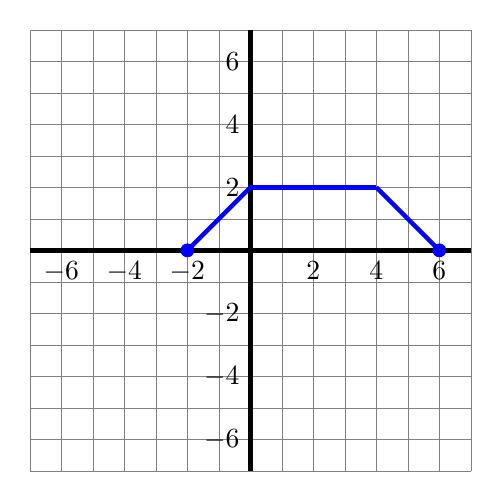
\begin{tikzpicture}[scale=0.4]
\draw[step=1cm,gray,very thin] (-7,-7) grid (7,7);
\draw[black,ultra thick] (-7,0) -- (7,0);
\draw[black,ultra thick] (0,-7) -- (0,7);

\foreach\x/\xtext in {-6,-4,-2,2,4,6}
\draw (\x ,1pt) -- (\x,-1pt) node[anchor=north] {$\xtext$};
\foreach\y/\ytext in {-6,-4,-2,2,4,6}
\draw (1pt,\y) -- (-1pt,\y) node[anchor=east] {$\ytext$};
\draw[blue,ultra thick] (-2,0) -- (0,2);
\draw[blue,ultra thick] (0,2) -- (4,2);
\draw[blue,ultra thick] (4,2) -- (6,0);
\node[circle,fill=blue,inner sep=0pt,minimum size=5pt](x) at (-2,-0) {};
\node[circle,fill=blue,inner sep=0pt,minimum size=5pt](y) at (6,0) {};
\end{tikzpicture}
\end{center}
\fi

\subsection{Describing transformations}

\begin{exercise}
Describe the graph of $y=3f(x-2)+4$ in terms of the graph
of $y=f(x)$.
\end{exercise}
\begin{solution}[1in]

\end{solution}

\begin{exercise}
Describe the graph of $y=\frac{1}{4}f(-x+2)$ in terms of the graph
of $y=f(x)$.
\end{exercise}
\begin{solution}[1in]

\end{solution}

\subsection{Graphing multiple transformations}

\begin{note}
Here is a rule of thumb for transformations:
\begin{itemize}
    \item Work inside to outside.
    \item Multiplication/division before addition/subtraction
\end{itemize}
\end{note}

\begin{exercise}
Graph $y=f(-x+3)-4$ using the graph of $y=f(x)$ below:
\end{exercise}
\ifprintanswers
\else
\begin{center}
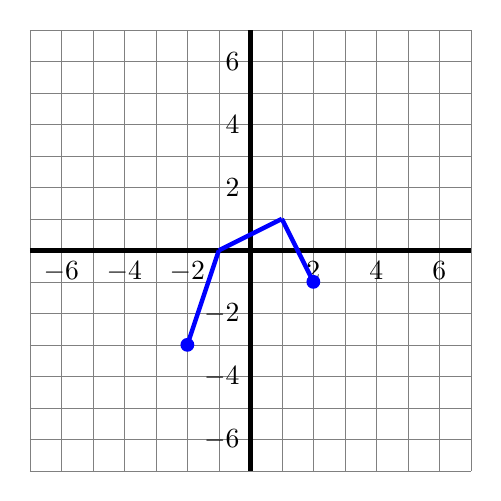
\begin{tikzpicture}[scale=0.4]
\draw[step=1cm,gray,very thin] (-7,-7) grid (7,7);
\draw[black,ultra thick] (-7,0) -- (7,0);
\draw[black,ultra thick] (0,-7) -- (0,7);

\foreach\x/\xtext in {-6,-4,-2,2,4,6}
\draw (\x ,1pt) -- (\x,-1pt) node[anchor=north] {$\xtext$};
\foreach\y/\ytext in {-6,-4,-2,2,4,6}
\draw (1pt,\y) -- (-1pt,\y) node[anchor=east] {$\ytext$};
\draw[blue,ultra thick] (-2,-3) -- (-1,0);
\draw[blue,ultra thick] (-1,0) -- (1,1);
\draw[blue,ultra thick] (1,1) -- (2,-1);
\node[circle,fill=blue,inner sep=0pt,minimum size=5pt](x) at (-2,-3) {};
\node[circle,fill=blue,inner sep=0pt,minimum size=5pt](y) at (2,-1) {};
\end{tikzpicture}
\end{center}
\fi
\begin{solution}[1in]

\end{solution}

\newpage

\begin{exercise}
Graph $y=3f(x+2)-1$ using the graph of $y=f(x)$ below:
\end{exercise}
\ifprintanswers
\else
\begin{center}
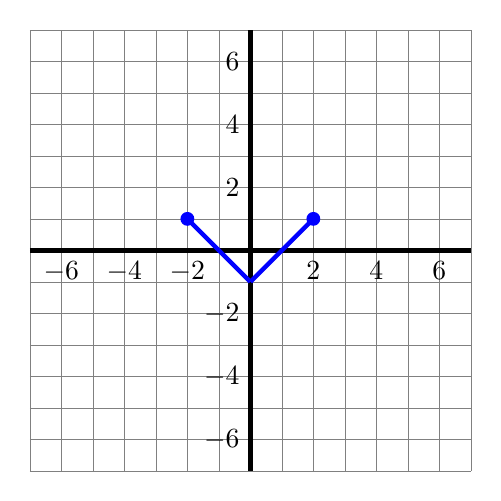
\begin{tikzpicture}[scale=0.4]
\draw[step=1cm,gray,very thin] (-7,-7) grid (7,7);
\draw[black,ultra thick] (-7,0) -- (7,0);
\draw[black,ultra thick] (0,-7) -- (0,7);

\foreach\x/\xtext in {-6,-4,-2,2,4,6}
\draw (\x ,1pt) -- (\x,-1pt) node[anchor=north] {$\xtext$};
\foreach\y/\ytext in {-6,-4,-2,2,4,6}
\draw (1pt,\y) -- (-1pt,\y) node[anchor=east] {$\ytext$};
\draw[blue,ultra thick] (-2,1) -- (0,-1);
\draw[blue,ultra thick] (0,-1) -- (2,1);
\node[circle,fill=blue,inner sep=0pt,minimum size=5pt](x) at (-2,1) {};
\node[circle,fill=blue,inner sep=0pt,minimum size=5pt](y) at (2,1) {};
\end{tikzpicture}
\end{center}
\fi
\begin{solution}[1in]

\end{solution}

\begin{exercise}
Graph $y=3f(2x-2)+2$ using the graph of $y=f(x)$ below:
\end{exercise}
\ifprintanswers
\else
\begin{center}
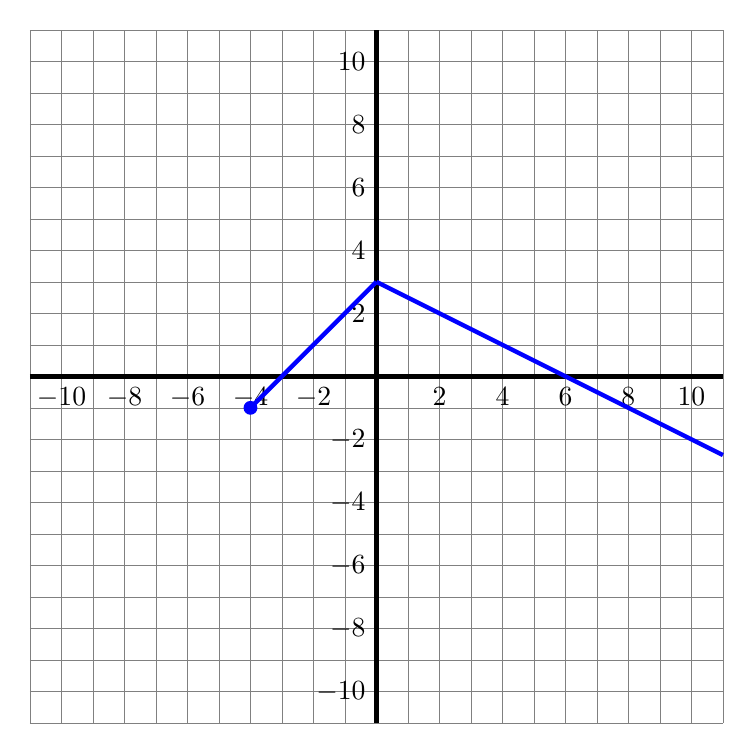
\begin{tikzpicture}[scale=0.4]
\draw[step=1cm,gray,very thin] (-11,-11) grid (11,11);
\draw[black,ultra thick] (-11,0) -- (11,0);
\draw[black,ultra thick] (0,-11) -- (0,11);

\foreach\x/\xtext in {-10,-8,-6,-4,-2,2,4,6,8,10}
\draw (\x ,1pt) -- (\x,-1pt) node[anchor=north] {$\xtext$};
\foreach\y/\ytext in {-10,-8,-6,-4,-2,2,4,6,8,10}
\draw (1pt,\y) -- (-1pt,\y) node[anchor=east] {$\ytext$};
\draw[blue,ultra thick] (-4,-1) -- (0,3);
\draw[blue,ultra thick] (0,3) -- (11,-5/2);
\node[circle,fill=blue,inner sep=0pt,minimum size=5pt](x) at (-4,-1) {};
\end{tikzpicture}
\end{center}
\fi
\begin{solution}[1in]

\end{solution}

\newpage

\begin{exercise}
Using $y=f(x)$ below, graph $y=f(-x-3)+1$
\end{exercise}
\ifprintanswers
\else
\begin{center}
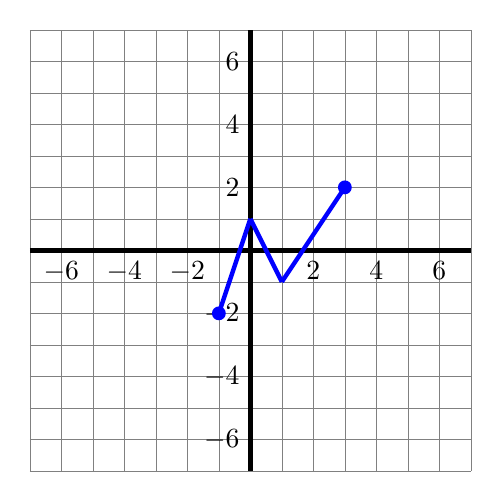
\begin{tikzpicture}[scale=0.4]
\draw[step=1cm,gray,very thin] (-7,-7) grid (7,7);
\draw[black,ultra thick] (-7,0) -- (7,0);
\draw[black,ultra thick] (0,-7) -- (0,7);

\foreach\x/\xtext in {-6,-4,-2,2,4,6}
\draw (\x ,1pt) -- (\x,-1pt) node[anchor=north] {$\xtext$};
\foreach\y/\ytext in {-6,-4,-2,2,4,6}
\draw (1pt,\y) -- (-1pt,\y) node[anchor=east] {$\ytext$};
\draw[blue,ultra thick] (-1,-2) -- (0,1);
\draw[blue,ultra thick] (0,1) -- (1,-1);
\draw[blue,ultra thick] (1,-1) -- (3,2);
\node[circle,fill=blue,inner sep=0pt,minimum size=5pt](x) at (-1,-2) {};
\node[circle,fill=blue,inner sep=0pt,minimum size=5pt](x) at (3,2) {};
\end{tikzpicture}
\end{center}
\fi
\begin{solution}[1in]

\end{solution}


\section{More on Functions \& Piece-wise Functions}

\subsection{Even and Odd Functions}

There are two ways to see whether a functions is even, odd or neither.

\subsubsection*{Algebraically}
\begin{definition}\label{def: even and odd functions}
\text{}
\begin{itemize}
    \item If $f(x)$ is odd, then $f(-x)=\blank{-f(x)}{-f(x)}$.
    \item If $f(x)$ is even, then $f(-x)=\blank{f(x)}{f(x)}$.
\end{itemize}
\end{definition}

\begin{exercise}
Is $f(x)=x^2+6$ even, odd, or neither?
\end{exercise}
\begin{solution}[2in]

\end{solution}
\vspace{0.5em}

\begin{exercise}
Is $g(x)=x^3-x$ even, odd, or neither?
\end{exercise}
\begin{solution}[2in]

\end{solution}
\vspace{0.5em}

\begin{exercise}
Is $h(x)=x^5+1$ even, odd, or neither?
\end{exercise}
\begin{solution}[2in]

\end{solution}
\vspace{0.5em}

Notice the following
\begin{itemize}
    \item $f(x)$ had all even powers.
    \item $g(x)$ had all odd powers.
    \item $h(x)$ had both even and odd powers.
\end{itemize}

\begin{fact}
\text{}
\begin{itemize}
    \item If all the powers in a polynomial are \blank{even}{even}, then it is as an even function.
    \item If all the powers in a polynomial are \blank{odd}{odd}, then it is as an odd function.
\end{itemize}
\end{fact}

\newpage

\subsubsection*{Graphically}

Recall that if $f(x)$ is even, then $f(-x)=f(x)$. This means that $x$
and $-x$ have the same value. So $f(x)$ is even if it has
\blank{$y$-axis symmetry}{$y$-axis symmetry}

\ifprintanswers
\else
\begin{center}
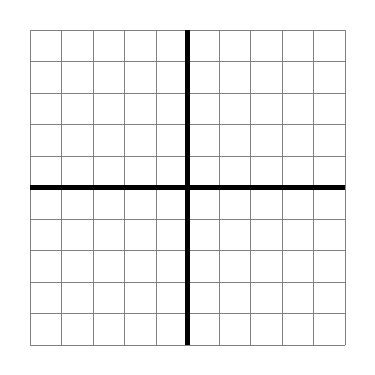
\begin{tikzpicture}[scale=0.4]
\draw[step=1cm,gray,very thin] (-5,-5) grid (5,5);
\draw[black,ultra thick] (-5,0) -- (5,0);
\draw[black,ultra thick] (0,-5) -- (0,5);
\end{tikzpicture}
\hspace{2in}
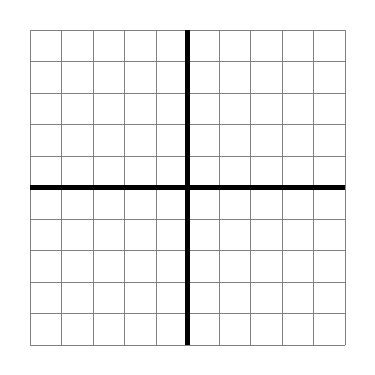
\begin{tikzpicture}[scale=0.4]
\draw[step=1cm,gray,very thin] (-5,-5) grid (5,5);
\draw[black,ultra thick] (-5,0) -- (5,0);
\draw[black,ultra thick] (0,-5) -- (0,5);
\end{tikzpicture}
\end{center}
\fi

If $f(x)$ is instead odd, then $f(-x)=-f(x)$. This means that $x$
and $-x$ have opposite values, so we say that $f(x)$ is odd if it
has \blank{origin symmetry}{symmetry}.

\ifprintanswers
\else
\begin{center}
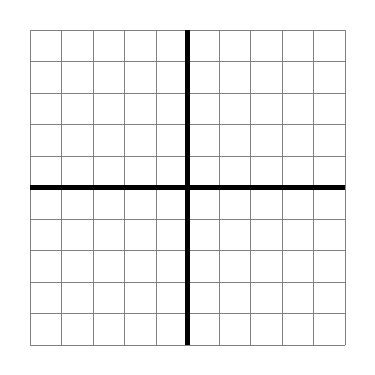
\begin{tikzpicture}[scale=0.4]
\draw[step=1cm,gray,very thin] (-5,-5) grid (5,5);
\draw[black,ultra thick] (-5,0) -- (5,0);
\draw[black,ultra thick] (0,-5) -- (0,5);
\end{tikzpicture}
\hspace{2in}
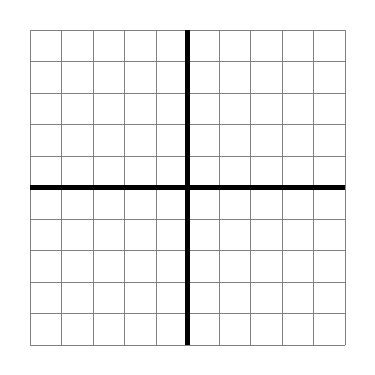
\begin{tikzpicture}[scale=0.4]
\draw[step=1cm,gray,very thin] (-5,-5) grid (5,5);
\draw[black,ultra thick] (-5,0) -- (5,0);
\draw[black,ultra thick] (0,-5) -- (0,5);
\end{tikzpicture}
\end{center}
\fi

\subsection{Piece-wise functions}

\begin{definition}\label{def: piecewise function}
A \emph{piece-wise defined function} or \emph{piece-wise} function
is a function that is defined by different functions on different
parts of its domain. Said another way, piece-wise functions are made
of ``pieces'' of other functions.
\end{definition}

\begin{example}
\[
f(x)=
\begin{cases}
2x-1 & \text{if }x<-1\\
x+1 & \text{if }x\geq-1
\end{cases}
\]
\end{example}

\newpage

\subsubsection*{Graphing}

\begin{exercise}
Graph
\[
f(x)=
\begin{cases}
2x-1 & \text{if }x<-1\\
x+1 & \text{if }x\geq-1
\end{cases}
\]
\end{exercise}
\ifprintanswers
\else
\begin{center}
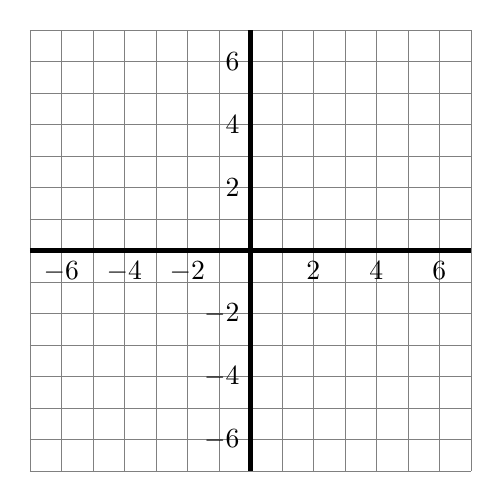
\begin{tikzpicture}[scale=0.4]
\draw[step=1cm,gray,very thin] (-7,-7) grid (7,7);
\draw[black,ultra thick] (-7,0) -- (7,0);
\draw[black,ultra thick] (0,-7) -- (0,7);

\foreach\x/\xtext in {-6,-4,-2,2,4,6}
\draw (\x ,1pt) -- (\x,-1pt) node[anchor=north] {$\xtext$};
\foreach\y/\ytext in {-6,-4,-2,2,4,6}
\draw (1pt,\y) -- (-1pt,\y) node[anchor=east] {$\ytext$};
\end{tikzpicture}
\end{center}
\fi
\begin{solution}[1in]

\end{solution}

\begin{exercise}
Graph
\[
g(x)=
\begin{cases}
\vert x\vert & \text{if }x\leq2\\
1 & \text{if }x>2
\end{cases}
\]
\end{exercise}
\ifprintanswers
\else
\begin{center}
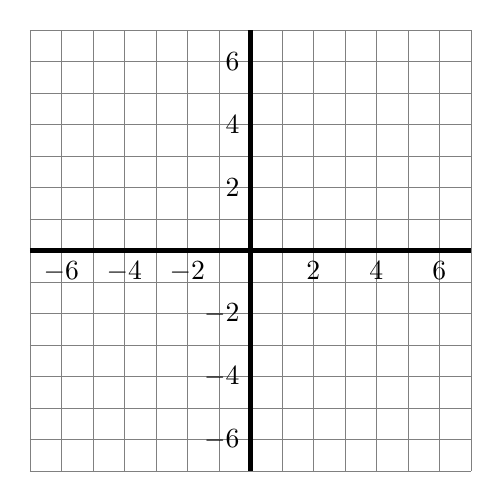
\begin{tikzpicture}[scale=0.4]
\draw[step=1cm,gray,very thin] (-7,-7) grid (7,7);
\draw[black,ultra thick] (-7,0) -- (7,0);
\draw[black,ultra thick] (0,-7) -- (0,7);

\foreach\x/\xtext in {-6,-4,-2,2,4,6}
\draw (\x ,1pt) -- (\x,-1pt) node[anchor=north] {$\xtext$};
\foreach\y/\ytext in {-6,-4,-2,2,4,6}
\draw (1pt,\y) -- (-1pt,\y) node[anchor=east] {$\ytext$};
\end{tikzpicture}
\end{center}
\fi
\begin{solution}[1in]

\end{solution}

\newpage

\subsubsection*{Evaluating}

\begin{exercise}
Find $f(2)$ for
\[
f(x)=
\begin{cases}
-2x & \text{if }x<1\\
x+2 & \text{if }1\leq x<3\\
x^2+2 & \text{if }3\leq x
\end{cases}
\]
\end{exercise}
\begin{solution}[2in]

\end{solution}

\vspace{0.5em}

\begin{exercise}
For
\[
g(x)=
\begin{cases}
-6x+4 & \text{if }x<3\\
3x-5 & \text{if } x\geq3
\end{cases}
\]
find $g(3)$.
\end{exercise}
\begin{solution}[2in]

\end{solution}

\ifprintanswers\else\newpage\fi

\section{Algebra of Functions}

\subsection{Basics}

Let $f(x)$ \& $g(x)$ be two functions and $D_f$ \& $D_g$ be their
domains

\begin{center}
\begin{tabular}{r|c}
Functions & Domains\\\hline
& \\
Sum: $(f+g)(x)=\blank{f(x)+g(x)}{f(x)+g(x)}$ & $\blank{D_f\cap D_g}{D_f \cap D_g}$\\
& \\
Difference: $(f-g)(x)=\blank{f(x)-g(x)}{f(x)-g(x)}$ & $\blank{D_f\cap D_g}{D_f\cap D_g}$\\
& \\
Product: $(fg)(x)=\blank{f(x)\cdot g(x)}{f(x)\cdot g(x)}$ & $\blank{D_f\cap D_g}{D_f\cap D_g}$\\
& \\
Quotient: $\dl\left(\frac{f}{g}\right)(x)=\blank{\frac{f(x)}{g(x)}}{\frac{f(x)}{g(x)}}$ & $\blank{D_f\cap D_g\setminus\{x\mid g(x)=0\}}{D_f\cap D_g\setminus\{x\mid g(x)=0\}}$
\end{tabular}
\end{center}

\begin{exercise}
For $f(x)=x^2-1$ \& $g(x)=3x-4$, find:
\end{exercise}
\ifprintanswers
\else
\begin{itemize}
    \item $(f+g)(x)=$
    \item $(f-g)(x)=$
    \item $(fg)(x)=$
    \item $\dl\left(\frac{f}{g}\right)(x)=$
\end{itemize}
\fi

\subsection{Composite Functions}

\begin{definition}\label{def: composite function}
Given two functions $f(x)$ and $g(x)$, the \emph{composition of $f$ and $g$} ($f$ compose $g$) is the following:
\[
(f\circ g)(x)=\blank{f(g(x))}{f(g(x))}
\]
\end{definition}
\vspace{0.5em}

\begin{exercise}
For $f(x)=4x+3$ and $g(x)=2x^2+5x$ find $(f\circ g)(x)$
\end{exercise}
\begin{solution}[1.5in]

\end{solution}
\vspace{0.5em}

\ifprintanswers\else\newpage\fi

\begin{exercise}
What if we found $(g\circ f)(x)$ instead?
\end{exercise}
\begin{solution}[1.5in]

\end{solution}
\vspace{0.5em}

\begin{exercise}
For $f(x)=6x-1$ and $g(x)=4x^2+x$, find both $(f\circ g)(x)$ and
$(g\circ f)(x)$.
\end{exercise}
\begin{solution}[2in]

\end{solution}
\vspace{0.5em}

\ifprintanswers\else\newpage\fi

\subsection{Evaluating compositions}

There are two ways evaluate compositions: algebraically \& graphically.

\subsubsection*{Algebraically}

\begin{exercise}
Given $f$ and $g$ below, find $f(g(3))$.
\begin{align*}
f(x)&=-4x-6\\
g(x)&=x-3
\end{align*}
\end{exercise}
\begin{solution}[3in]

\end{solution}
\vspace{0.5em}

\begin{exercise}
Find $(f\circ g)(2)$ if $f(x)=-2x^2+4x+6$ \& $g(x)=2x-3$.
\end{exercise}
\begin{solution}[2in]

\end{solution}
\vspace{0.5em}

\ifprintanswers\else\newpage\fi

\subsubsection*{Graphically}

This will be very similar to the second algebraic technique.

\begin{exercise}
Find $f(g(2))$ using the graphs of $f$ and $g$ below:
\begin{center}
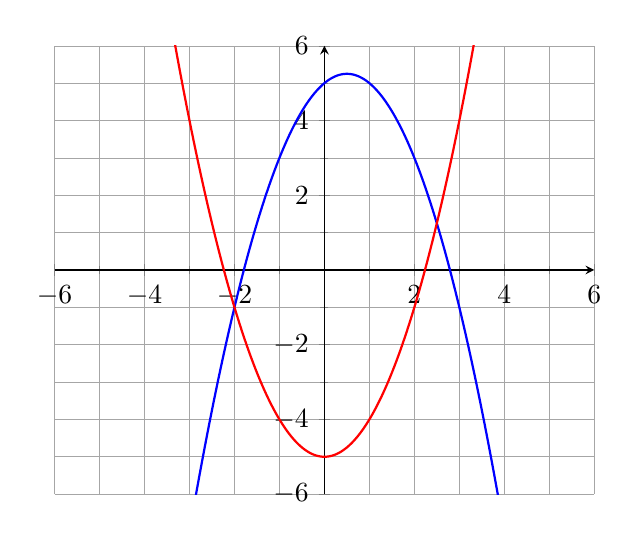
\begin{tikzpicture}
     \begin{axis}%
    [grid=both,
    ymin=-6, ymax=6,
    xmin=-6, xmax=6,
     minor tick num=1,
     grid style={line width=.2pt, draw=gray!70},
     major grid style={line width=.2pt,draw=gray!70},
     axis lines=middle,
     enlargelimits=false
    ]
    \addplot+[blue,mark=none,thick,samples=400] {-x^2+x+5};
    \addplot+[red,mark=none,thick,samples=400] {x^2-5};
  \end{axis}
\end{tikzpicture}
\end{center}
\end{exercise}
\begin{solution}[2in]

\end{solution}

\newpage

\subsection{Domains of Compositions}

Here is a nice visualization of compositions to understand their domains.

\ifprintanswers
\else
\vspace{4in}
\fi

\begin{fact}
If we have two functions $f(x)$ and $g(x)$ with $D_f$ and $D_g$ their
respective domains, then the domain of $(f\circ g)(x)$ is
\[
D_{f\circ g}=\blank{D_g\cap\{x\mid g(x)
\text{ is in }D_f\}}{D_g\cap\{x\mid g(x)\text{ is in }D_f\}}
\]
\end{fact}

\begin{exercise}
Find the domain of $(f\circ g)(x)$ when
\[
f(x)=\frac{1}{8x-16}\quad\&\quad g(x)=\sqrt{2x+10}
\]
\end{exercise}
\begin{solution}[2.5in]

\end{solution}

\begin{exercise}
Find the domain of $f(g(x))$ when
\[
f(x)=\frac{4}{x+2}\quad\&\quad g(x)=\frac{-2}{3x-2}
\]
\end{exercise}
\begin{solution}[2.5in]

\end{solution}

\subsection{Decomposing functions}

\begin{exercise}
Find $f(x)$ and $g(x)$ such that
\[
(f\circ g)(x)=\sqrt{x^2+1}
\]
\end{exercise}
\begin{solution}[3in]

\end{solution}

\newpage

\begin{exercise}
For $\dl h(x)=\frac{-5}{(-x-3)^9}$, find $f(x)$ and $g(x)$ such that
$f(g(x))=h(x)$.
\end{exercise}
\begin{solution}[3in]

\end{solution}